% arara: pdflatex: { shell: yes }
\documentclass{article}
\usepackage{graphicx}
\usepackage{booktabs}
\usepackage{float}

\title{Virtual Machines}
\author{Erick Gonzalez Parada ID: 178145}
\date{\today}

\begin{document}

\maketitle

\section{Introduction}
This document presents the results of the process of installing a Linux virtual machine with VirtualBox, what was necessary to get web browsing working or create a file, and a comparison between this virtual machine and the native operating system.

\section{Methodology}
First, we have to choose a Linux operating system. There are several flavors of Linux distributions, most of them aiming to be the best at some task, such as personalization, security, cybersecurity, serving, etc. In this case, I chose openSUSE OS because it is minimalistic, gets the job done, and is very stable and popular in the world of Linux distros.

Next, we need to find and download the ISO file, which can be found on the official webpage of the distro. There are several formats and mirrors available for downloading the image.

\begin{figure}[H]
	\centering
	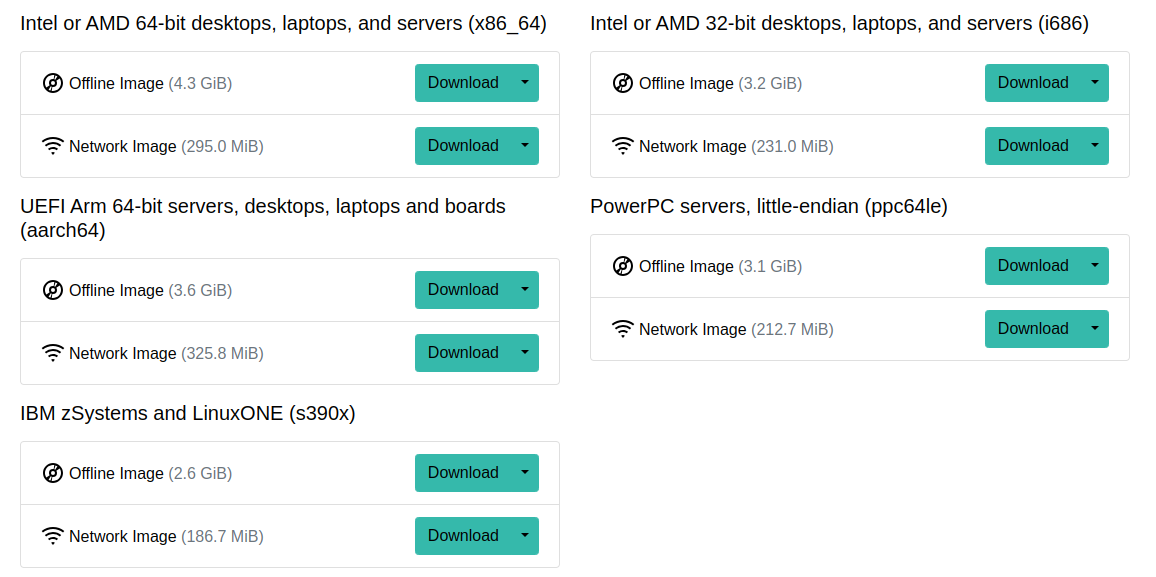
\includegraphics[width=1\textwidth]{iso.png}
	\caption{Download Formats}
	\label{fig:1}
\end{figure}

If VirtualBox software is not already installed, it should be downloaded. The app is available for Windows, Mac, and Linux, so one can have Linux on Linux, Windows on Mac, or any combination desired.

\begin{figure}[H]
	\centering
	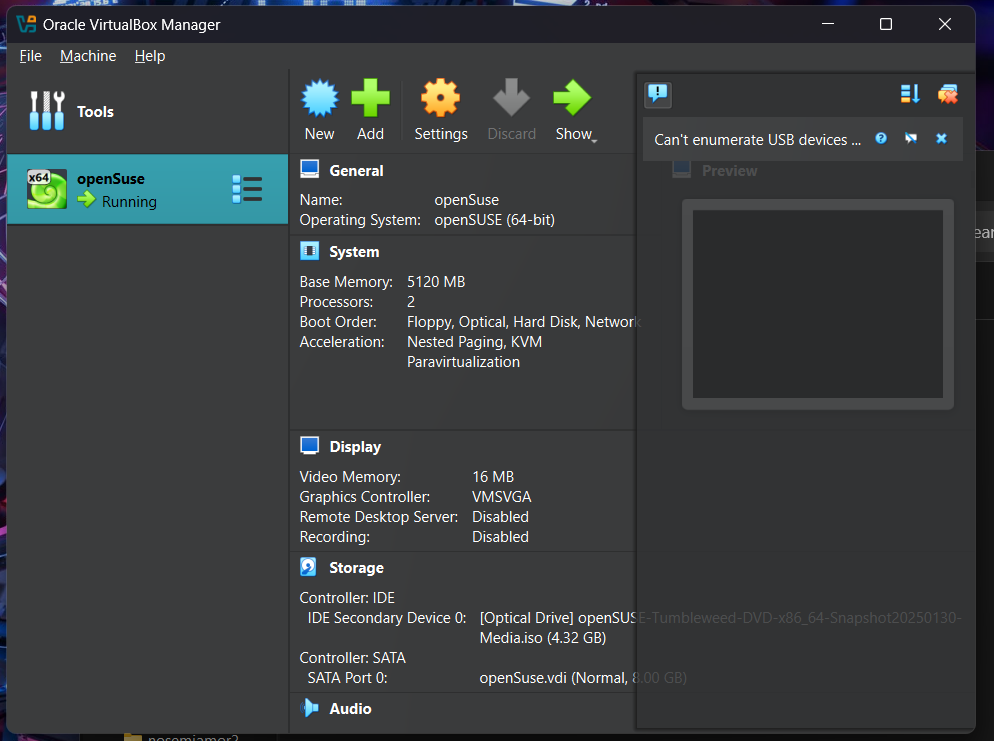
\includegraphics[width=1\textwidth]{vbx.png}
	\caption{VirtualBox Interface}
	\label{fig:2}
\end{figure}

Pressing the "New" button in the VM (virtual machine) manager allows processing the ISO file and allocating resources to the VM. In this case, I allocated 5 GB of RAM and 2 CPU cores.

\begin{figure}[H]
	\centering
	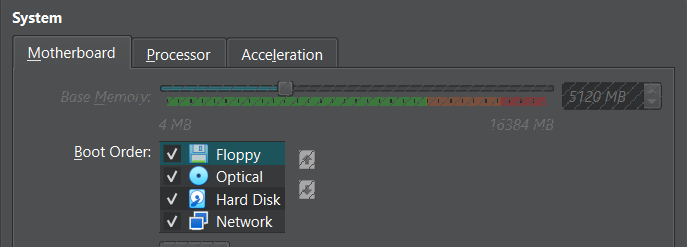
\includegraphics[width=1\textwidth]{ram.png}
	\caption{RAM Allocated}
	\label{fig:3}
\end{figure}

\begin{figure}[H]
	\centering
	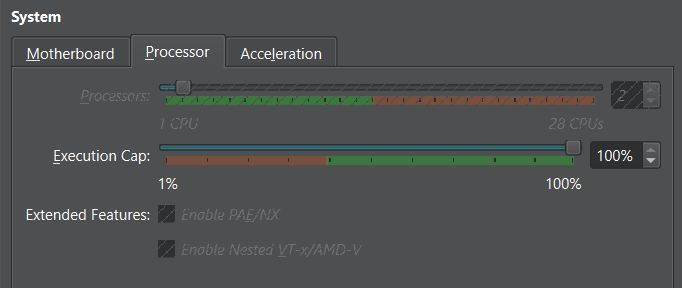
\includegraphics[width=1\textwidth]{core.png}
	\caption{CPUs Allocated}
	\label{fig:4}
\end{figure}

Finally, we can run the VM and start executing basic commands to check Wi-Fi connectivity, update the system, and install software like Chromium.

\begin{figure}[H]
	\centering
	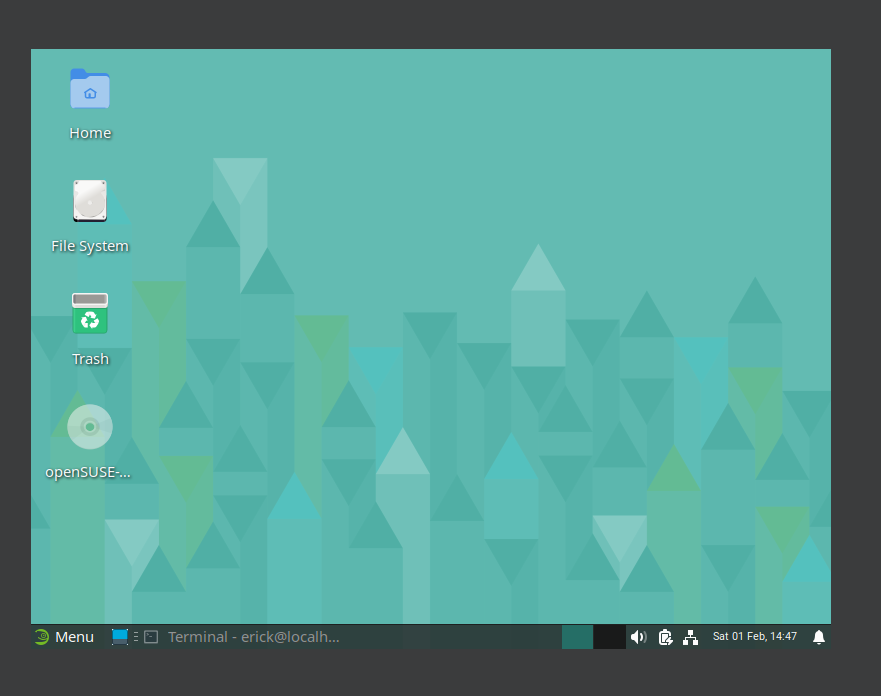
\includegraphics[width=1\textwidth]{wm.png}
	\caption{Logged In}
	\label{fig:5}
\end{figure}

\begin{figure}[H]
	\centering
	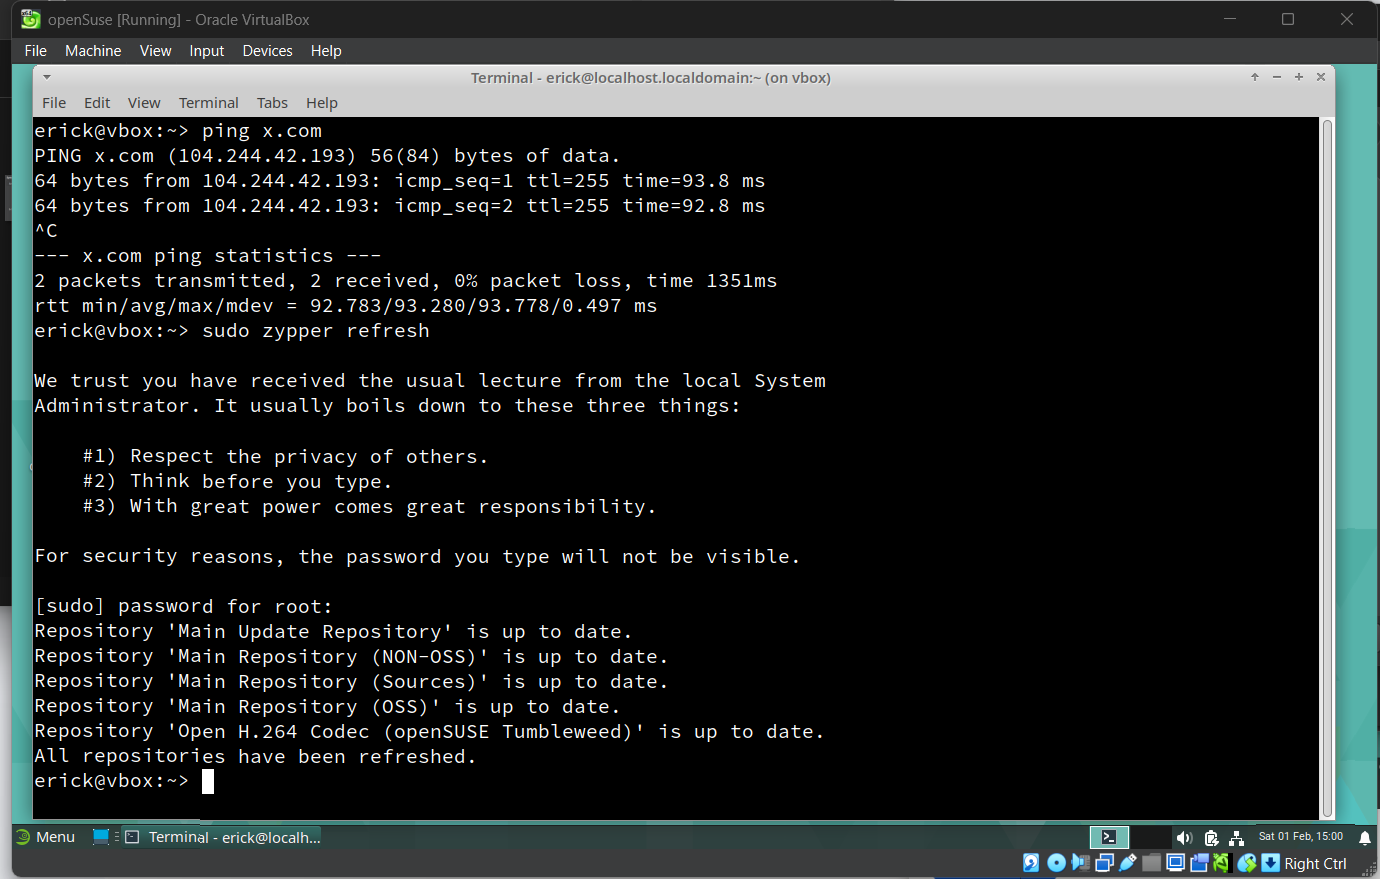
\includegraphics[width=1\textwidth]{su.png}
	\caption{Checking Wi-Fi and Updating}
	\label{fig:6}
\end{figure}

\begin{figure}[H]
	\centering
	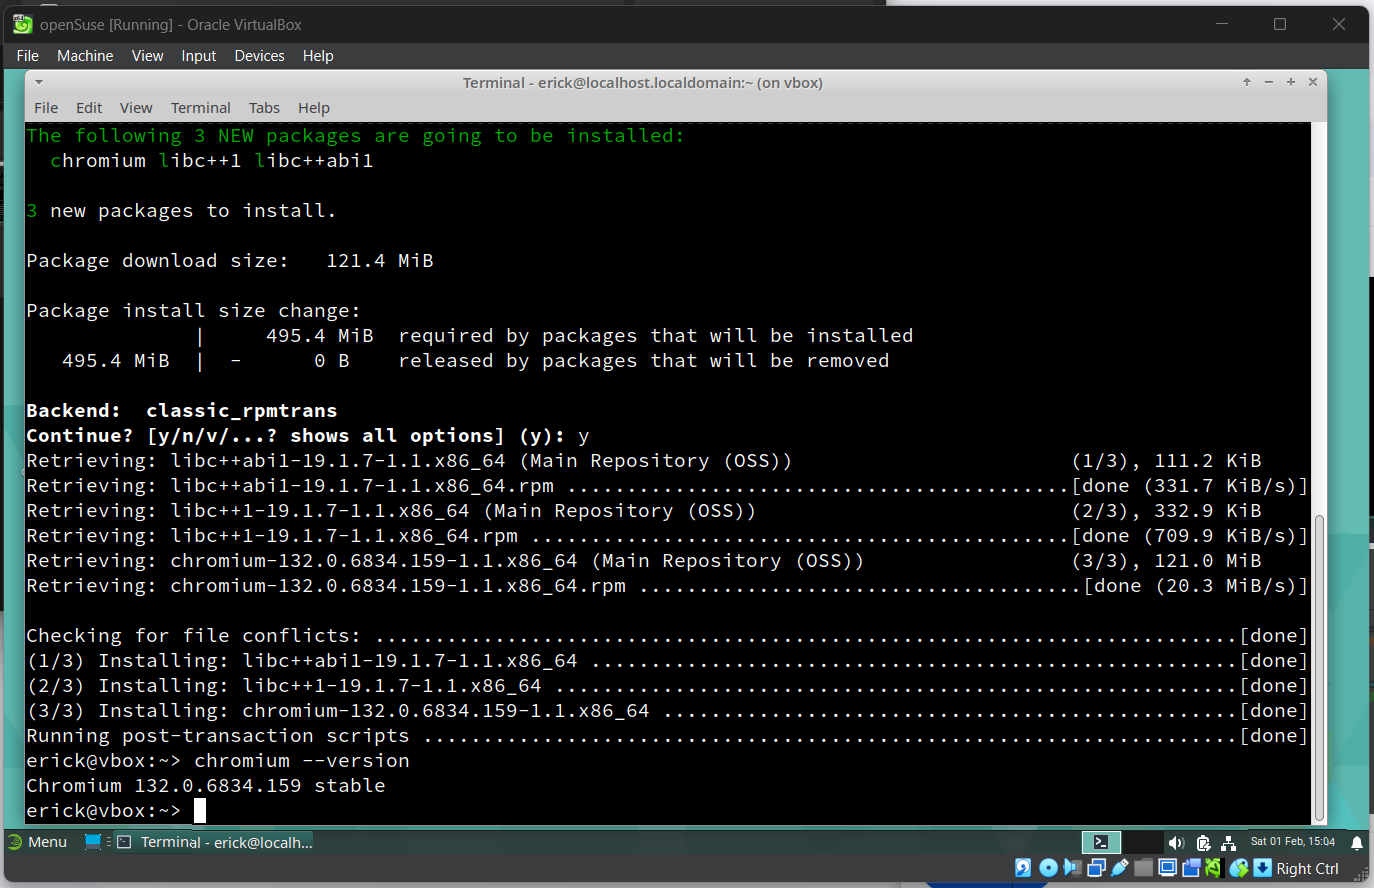
\includegraphics[width=1\textwidth]{chr.png}
	\caption{Installing Chromium}
	\label{fig:7}
\end{figure}

\section{Comparative Analysis}

\begin{table}[H]
    \centering
    \caption{Comparison Between Windows (Native) and openSUSE (VM)}
    \label{tab:comparison}
    \begin{tabular}{@{}lll@{}}
    \toprule
    \textbf{Aspect} & \textbf{Windows (Native)} & \textbf{openSUSE (VM)} \\
    \midrule
    \textbf{Performance} & Faster due to direct hardware access & Slightly slower due to virtualization overhead \\
    \textbf{Resource Usage} & Utilizes full system resources & Limited by allocated VM resources (5 GB RAM, 2 CPUs) \\
    \textbf{Software Installation} & Uses GUI or PowerShell & Relies on terminal commands (e.g., \texttt{zypper}) \\
    \textbf{Customization} & Limited customization options & Highly customizable, tailored to user needs \\
    \textbf{Stability} & Stable for general use & Very stable, designed for reliability \\
    \textbf{Use Case} & Ideal for general-purpose tasks & Great for development, testing, and learning Linux \\
    \bottomrule
    \end{tabular}
\end{table}

\section{Conclusion}
In conclusion, while Windows as a native system offers better performance and ease of use for general tasks, openSUSE in a virtual machine provides a highly customizable and stable environment for development and learning. The choice between the two depends on the user's needs: Windows for everyday use and openSUSE for specialized tasks and experimentation.

\section{References}
No references were used in this article.

\end{document}
